\documentclass[parskip=full]{scrartcl}
\usepackage[T1]{fontenc}    % avoid garbled Unicode text in pdf
\usepackage[utf8]{inputenc} % use utf8 file encoding for TeX sources
\usepackage[german]{babel}  % german hyphenation, quotes, etc
\usepackage{hyperref}       % detailed hyperlink/pdf configuration
\hypersetup{                % ‘texdoc hyperref‘ for options
pdftitle={PSE: Entwicklung eines relationalen Debuggers - Pflichtenheft},%
,%
}
\usepackage{graphicx}       % provides commands for including figures
\usepackage{csquotes}       % provides \enquote{} macro for "quotes"
\usepackage[nonumberlist]{glossaries}     % provides glossary commands
\usepackage{enumitem}

\makenoidxglossaries


\title{PSE:\\ Entwicklung eines relationalen Debuggers\\ Pflichtenheft}
\author{
	Benedikt Wagner\\
	\texttt{udpto@student.kit.edu}
	\and Chiara Staudenmaier\\
	\texttt{uzhtd@student.kit.edu}
	\and Étienne ?\\
	\texttt{urmlp@student.kit.edu}
	\and Joana Plewnia\\
	\texttt{uhfpm@student.kit.edu} 
	\and Pascal Zwick\\
	\texttt{uyqpk@student.kit.edu}
	\and Ulla Scheler\\
	\texttt{ujuhe@student.kit.edu}
}

\begin{document}

\maketitle
\newpage

\section{Produktübersicht}
%kurze Übersicht über das Produkt
..

\section{Produkteinsatz}
%Anwendungsbereiche, Zielgruppen, Betriebsbedingungen
..

\section{Produktumgebung}
%Software, Hardware, Orgware, Schnittstellen
..

\section{Produktfuntionen}
	\subsection{Funktionale Anforderungen}
		\subsubsection{Musskriterien}
		..
		\subsubsection{Sollkriterien}
		..
		\subsubsection{Kannkriterien}
		..
		\subsubsection{Abgrenzungskriterien}
		..
	\subsection{Nichtfunktionale Anforderungen}
		\subsubsection{Produktdaten}
		..
		\subsubsection{Produktleistungen}
		..
		\subsubsection{Weitere nichtfunktionale Anforderungen}
		..

\section{Qualitätsanforderungen}
..

\section{Anwendungsfälle und Szenarien}
\begin{figure}[h] 
  \centering
     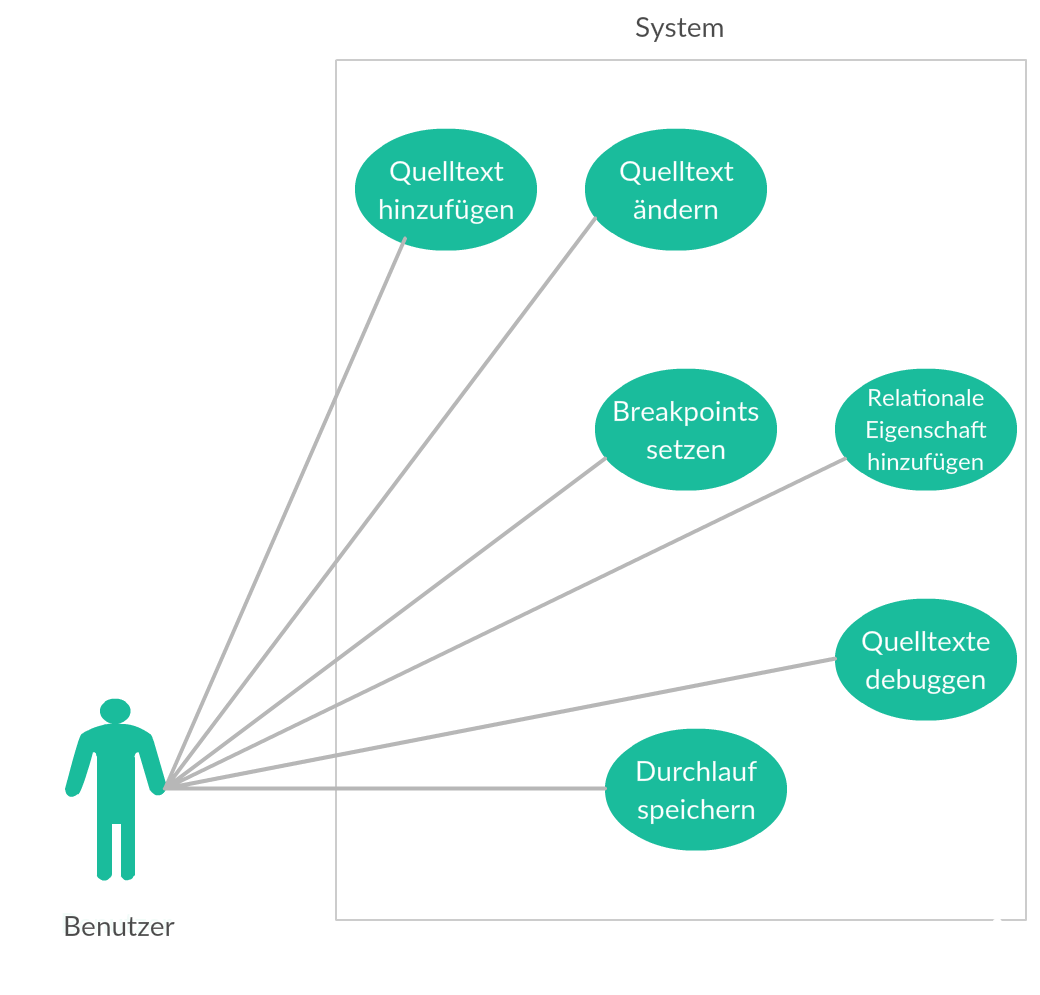
\includegraphics[width=0.7\textwidth]{Anwendungsfalldiagramm}
  \caption{Anwendungsfalldiagramm}
  \label{fig:Bild1}
\end{figure}

\section{Globale Testfälle}
..

\section{Systemmodelle}
%Architektur, Verhalten, usw
\begin{figure}[h] 
  \centering
     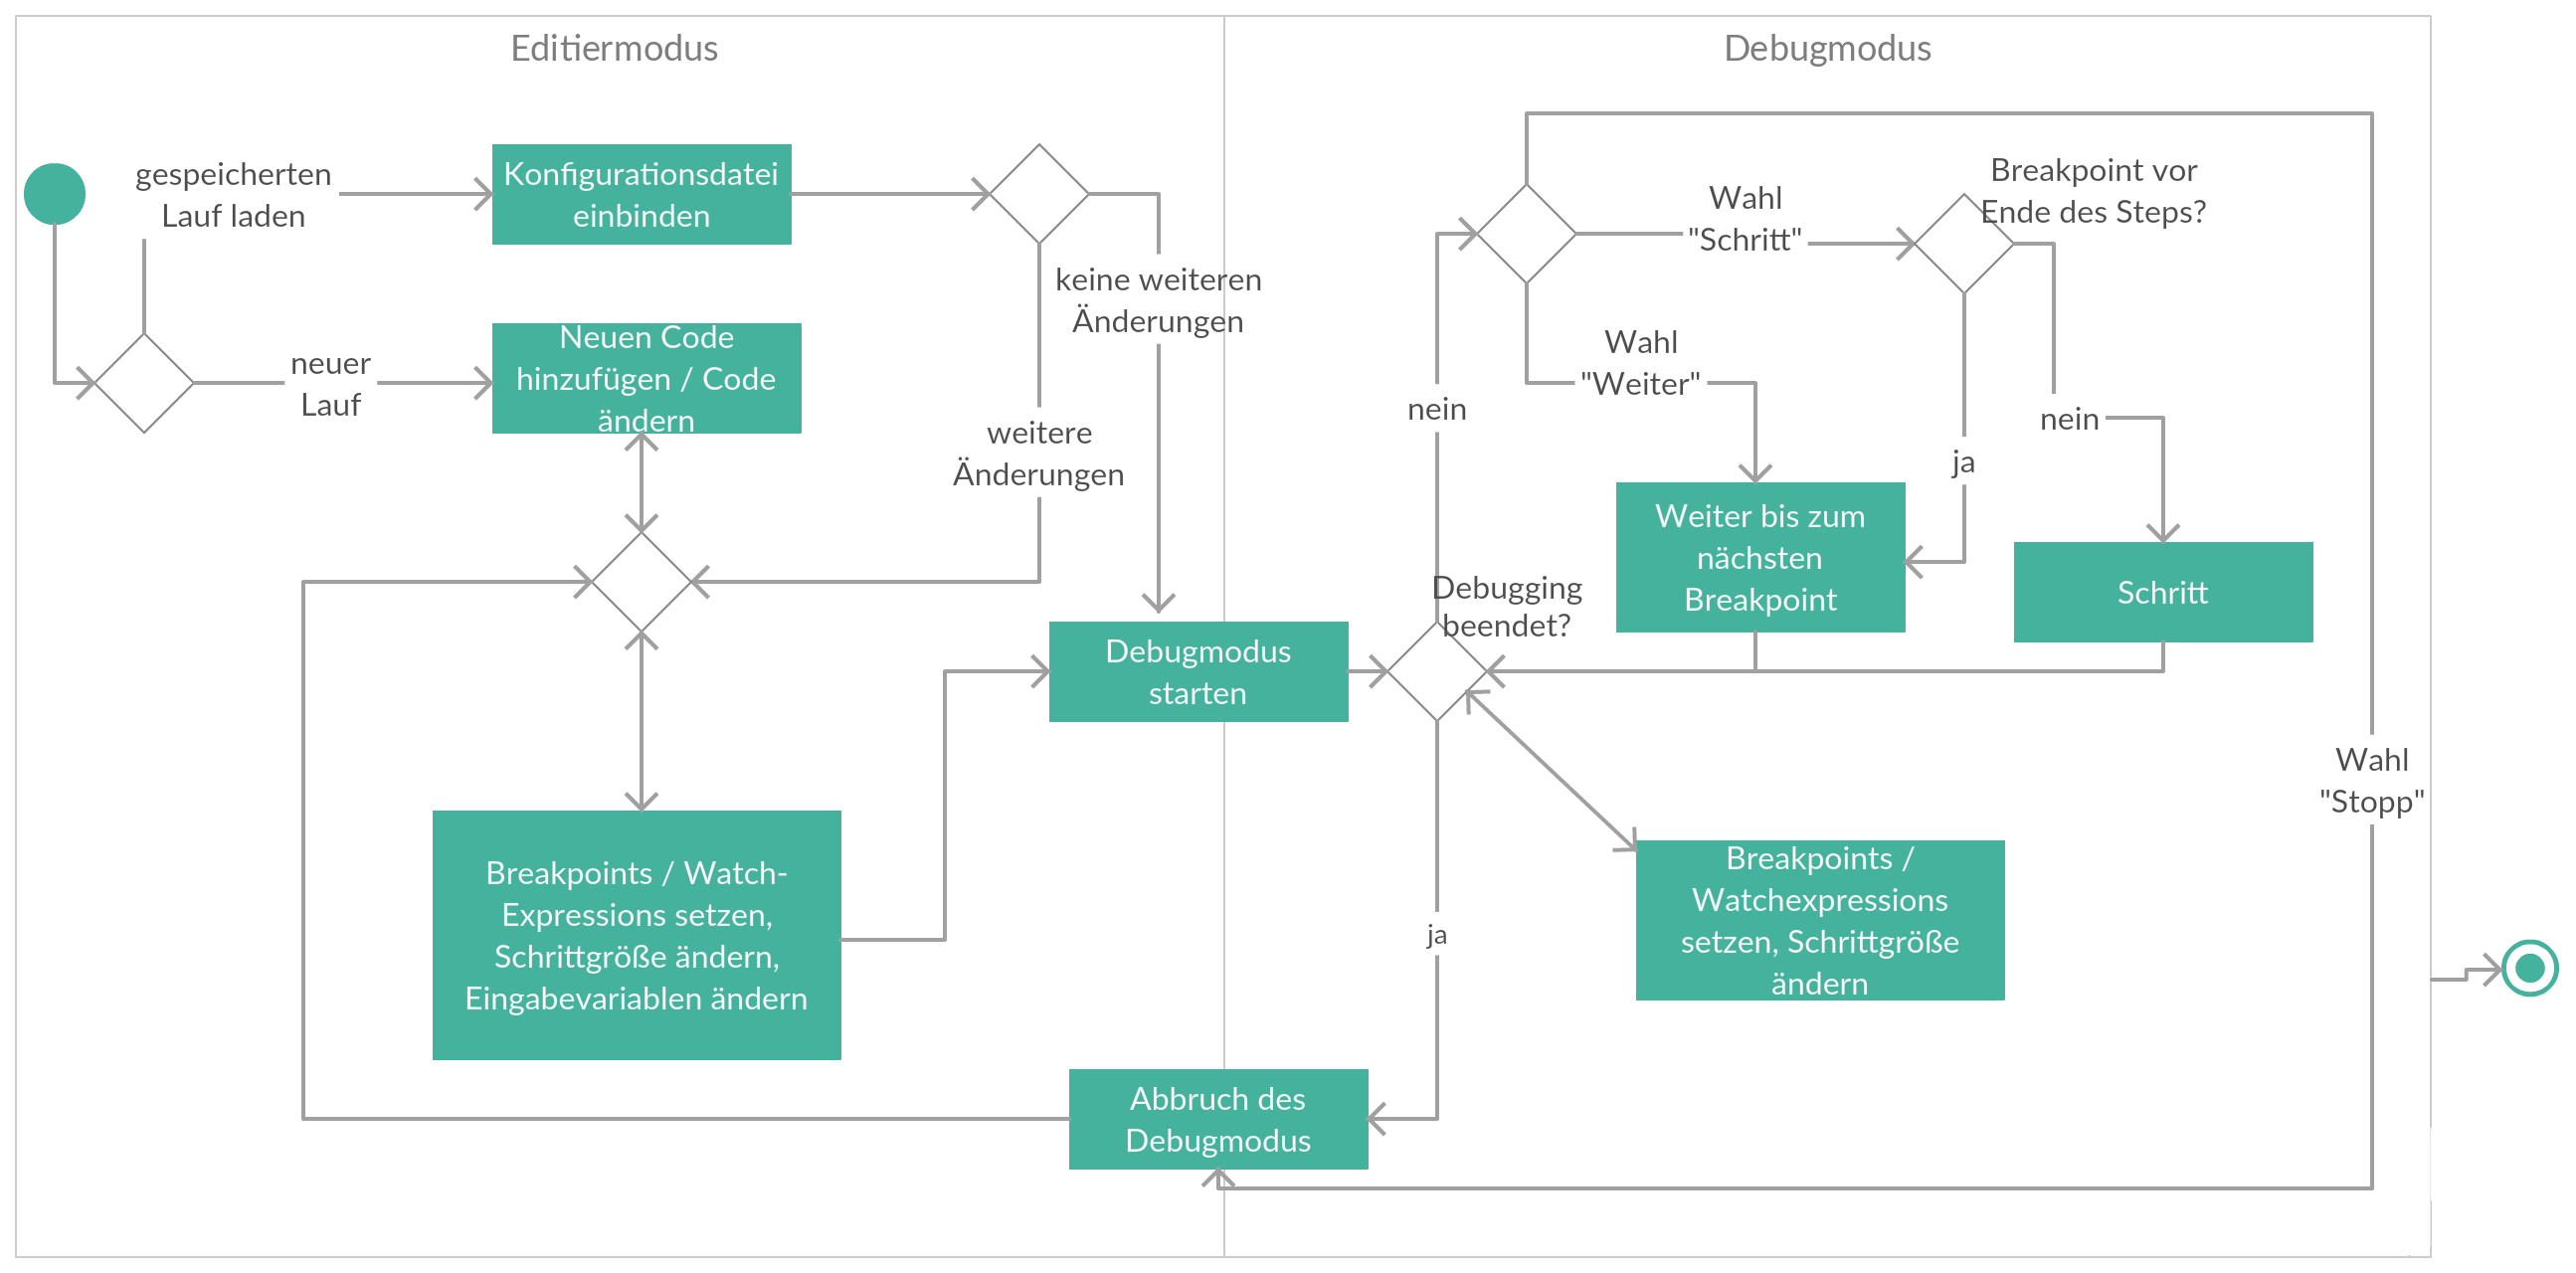
\includegraphics[width=0.9\textwidth]{Aktivitaetsdiagramm}
  \caption{Aktivitätsdiagramm}
  \label{fig:Bild1}
\end{figure}


\section{Benutzungsoberfläche}
%Gui-Skizzen, Erklärungen der Menüs, usw
..

\section{Zeit- und Ressourcenplanung}
..

\section{Ergänzungen}
..

\section{Glossar}




\end{document}
\grid
